\documentclass[12pt]{scrartcl}

\usepackage{amsmath,amssymb}
\usepackage{fullpage}
\usepackage{enumitem}
\usepackage{hyperref}
\usepackage{graphicx}
\usepackage{tikz}
\usepackage{pgfplots}
\usepackage{float}
\usepackage{tabularx}
\usepackage{titlesec}

\pgfplotsset{compat=1.18}
\usetikzlibrary{trees,positioning,shapes,arrows}
\usepgfplotslibrary{statistics} 
\setlength{\parindent}{0pt}

\tikzset{
  basic/.style  = {draw, text width=2cm, drop shadow, font=\sffamily, rectangle},
  root/.style   = {basic, rounded corners=2pt, thin, align=center, fill=white},
  level-2/.style = {basic, rounded corners=6pt, thin,align=center, fill=white, text width=4cm},
  level-3/.style = {basic, thin, align=center, fill=white, text width=3cm}
}

\titleformat{\section}  % which section command to format
{\fontsize{12}{14}\bfseries} % format for whole line
{\thesection} % how to show number
{1em} % space between number and text
{} % formatting for just the text
[] % formatting for after the text

\titleformat{\subsection}  % which section command to format
{\fontsize{12}{14}\bfseries} % format for whole line
{\thesubsection} % how to show number
{1em} % space between number and text
{} % formatting for just the text
[] % formatting for after the text

\begin{document}

\begin{center}
	\hrule
	\vspace{0.4cm}
	{\textbf{\large Lecture 04: Continuous Probability Distributions}} \\ [0.2cm]
	INF1004 Mathematics II

\end{center}

\textbf{Name:} Timothy Chia \hspace{\fill} \textbf{Date:} 26/03/2025 \\

\hrule

\section{Introduction}

In our previous study of discrete random variables, we dealt with countable outcomes, such as the number of heads in a series of coin flips. However, many real-world phenomena---such as time, weight, or distance---exist in a continuous space where an infinite number of values are possible within any given range. 

\begin{figure}[H]
	\centering
	\begin{minipage}{0.55\textwidth}
		\centering
		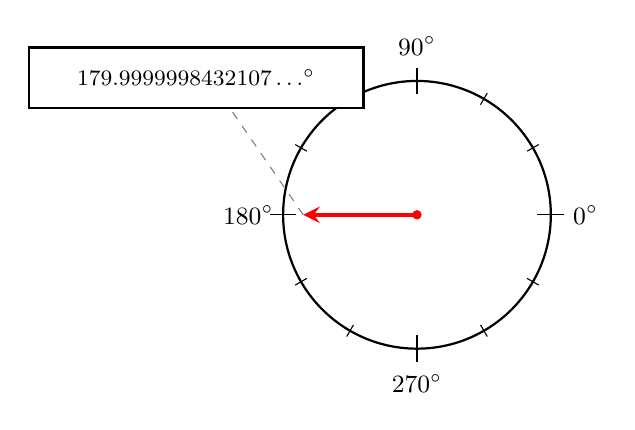
\begin{tikzpicture}[scale=0.85]
			\draw[thick] (0,0) circle (2cm);
			\foreach \a in {0, 90, 180, 270}
				\draw (\a:1.8cm) -- (\a:2.2cm) node[pos=1.8] {\small\a$^\circ$};
			\foreach \a in {30, 60, 120, 150, 210, 240, 300, 330}
				\draw (\a:1.9cm) -- (\a:2.1cm);
 
			\draw[->, >=stealth, ultra thick, red] (0,0) -- (179.9999998:1.7cm);
			\fill[red] (0,0) circle (2pt);
 
			\draw[dashed, gray] (180:1.7cm) -- (-2.8, 1.6);
			\draw[fill=white, thick] (-5.8, 1.6) rectangle (-0.8, 2.5);
			\node at (-3.3, 2.05) {\footnotesize $179.9999998432107\dots^\circ$};
 
			% \draw[thick, gray] (180:2.0cm) circle (0.28cm);
		\end{tikzpicture}
	\end{minipage}\hfill
	\begin{minipage}{0.40\textwidth}
		\centering
		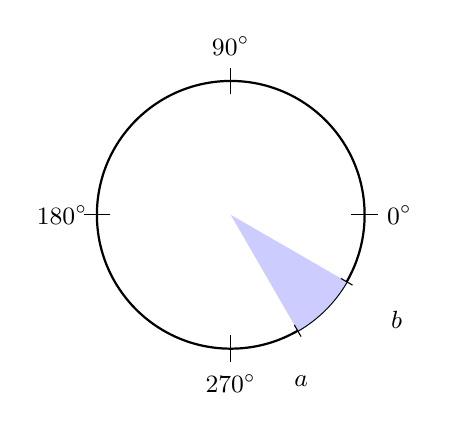
\begin{tikzpicture}[scale=0.85]
			\draw[thick] (0,0) circle (2cm);
			\fill[blue!20] (0,0) -- (300:2cm) arc (300:330:2cm) -- cycle;
			\foreach \a in {0, 90, 180, 270}
				\draw (\a:1.8cm) -- (\a:2.2cm) node[pos=1.8] {\small\a$^\circ$};
			\draw (300:1.9cm) -- (300:2.1cm);
			\draw (330:1.9cm) -- (330:2.1cm);
			\node[below left]  at (300:2.6cm) {\small $a$};
			\node[below right] at (330:2.6cm) {\small $b$};
		\end{tikzpicture}
	\end{minipage}
	\caption{Infinite precision in a continuous space.}
\end{figure}

A fundamental, yet counter-intuitive, property of continuous spaces is that the probability of a random variable taking an exact, precise value is zero. Consider a spinning arrow on a circular board marked from 0 to 360 degrees. While the arrow must stop at some point, the probability that it stops at exactly $179.9999998^\circ$ (to infinite precision) is effectively zero. Because there are infinitely many points on the circle, the likelihood of hitting one specific point is negligible. Consequently, in continuous probability, we shift our focus from individual points to the probability of the variable falling within a specific interval.

\section{The Probability Density Function (PDF)}

To describe the behavior of a continuous random variable $X$, we use a Probability Density Function, denoted as $f(x)$. Unlike the probability mass function of a discrete variable, $f(x)$ does not represent a probability directly; instead, it represents the ``density'' of the probability at a specific point. \\

The probability that $X$ falls within the interval $[a, b]$ is defined as the area under the curve of $f(x)$ between those two points. Mathematically, this is expressed using the integral:
\begin{equation}
	P(a \le X \le b) = \int_{a}^{b} f(x) \, dx
\end{equation}

For a function to be a valid PDF, it must satisfy two primary conditions: the density must be non-negative for all values ($f(x) \ge 0$), and the total area under the entire curve must equal exactly one:
\begin{equation}
	\int_{-\infty}^{\infty} f(x) \, dx = 1
\end{equation}

\begin{figure}[H]
	\centering
	% TIKZ_PLACEHOLDER_2: A generic continuous curve with a shaded region between vertical lines at points a and b.
	\begin{tikzpicture}
		\begin{axis}[
			axis lines = left,
			xlabel = $x$,
			ylabel = $f(x)$,
			ymin=0, ymax=0.5,
			xmin=0, xmax=6,
			ticks=none,
			domain=0:6,
			samples=100,
			height=5cm, width=8cm
		]
			\addplot [name path=curve, thick, blue] {0.4*exp(-(x-3)^2/2.5)};
			
			\addplot [
				fill=blue,
				fill opacity=0.2,
				domain=1.5:4.5
			] {0.4*exp(-(x-3)^2/2.5)} \closedcycle;
			
			\draw[dashed] (axis cs:1.5, 0) -- (axis cs:1.5, {0.4*exp(-(1.5-3)^2/2.5)}) node[below, pos=0] {$a$};
			\draw[dashed] (axis cs:4.5, 0) -- (axis cs:4.5, {0.4*exp(-(4.5-3)^2/2.5)}) node[below, pos=0] {$b$};
			
			\node at (axis cs:3, 0.15) {$P(a \le X \le b)$};
		\end{axis}
	\end{tikzpicture}
	\caption{Probability as the area under the density curve.}
\end{figure}

\section{The Continuous Uniform Distribution}

The simplest continuous distribution is the Uniform Distribution, often referred to as the rectangular distribution. This model is used when every interval of the same length within the distribution's support is equally probable. If a variable $X$ is uniformly distributed over the interval $[a, b]$, its density function is constant:
\begin{equation}
	f(x) = \frac{1}{b - a} \quad \text{for } a \le x \le b
\end{equation}

Returning to our spinning arrow example (from $0^\circ$ to $360^\circ$), the density is $f(x) = 1/360$. The probability of the arrow stopping between $260^\circ$ and $290^\circ$ is simply the ratio of the width of that interval to the total width:
\begin{equation}
	P(260 \le X \le 290) = \frac{290 - 260}{360} = \frac{30}{360} = \frac{1}{12}
\end{equation}

\begin{figure}[H]
	\centering
	% TIKZ_PLACEHOLDER_3: A rectangular probability density plot over the interval [a, b] with height 1/(b-a).
	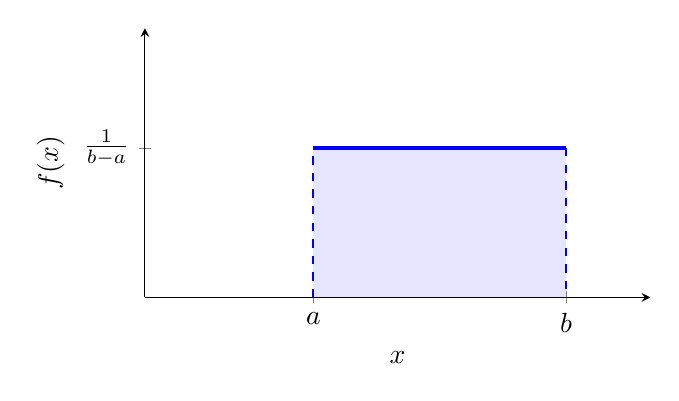
\begin{tikzpicture}
		\begin{axis}[
			axis lines = left,
			xlabel = $x$,
			ylabel = $f(x)$,
			ymin=0, ymax=0.6,
			xmin=0, xmax=6,
			xtick={2, 5},
			xticklabels={$a$, $b$},
			ytick={0.333},
			yticklabels={$\frac{1}{b-a}$},
			height=5cm, width=8cm
		]
			\addplot[ultra thick, blue, domain=2:5] {1/3};
			\addplot[thick, blue, dashed] coordinates {(2,0) (2, 0.333)};
			\addplot[thick, blue, dashed] coordinates {(5, 0.333) (5, 0)};
			\fill[blue, opacity=0.1] (axis cs:2,0) rectangle (axis cs:5,0.333);
		\end{axis}
	\end{tikzpicture}
	\caption{Uniform distribution over an interval $[a, b]$.}
\end{figure}

\section{The Normal Distribution}

The Normal Distribution, characterized by its iconic bell-shaped curve, is perhaps the most significant distribution in statistics due to its ability to model many natural phenomena. It is defined by two parameters: the mean ($\mu$), which determines the center of the distribution, and the variance ($\sigma^2$), which determines its spread. We denote this as $X \sim N(\mu, \sigma^2)$. \\

Because the mathematical formula for the normal density is complex, we often simplify problems by transforming the general normal variable $X$ into the Standard Normal Distribution, denoted as $Z$, where the mean is 0 and the variance is 1 ($Z \sim N(0, 1)$). This transformation is achieved using the Z-score formula:
\begin{equation}
	Z = \frac{X - \mu}{\sigma}
\end{equation}

By converting to $Z$, we can use standardized Z-tables to find probabilities. The symmetry of the normal curve allows us to derive various probabilities easily; for instance, $P(Z > z) = 1 - P(Z < z)$, and due to its symmetry around zero, $P(Z < -z) = P(Z > z)$.

\begin{figure}[H]
	\centering
	% TIKZ_PLACEHOLDER_4: A bell curve showing the transformation from a general X axis with mean $\mu$ to a Z axis with mean 0.
	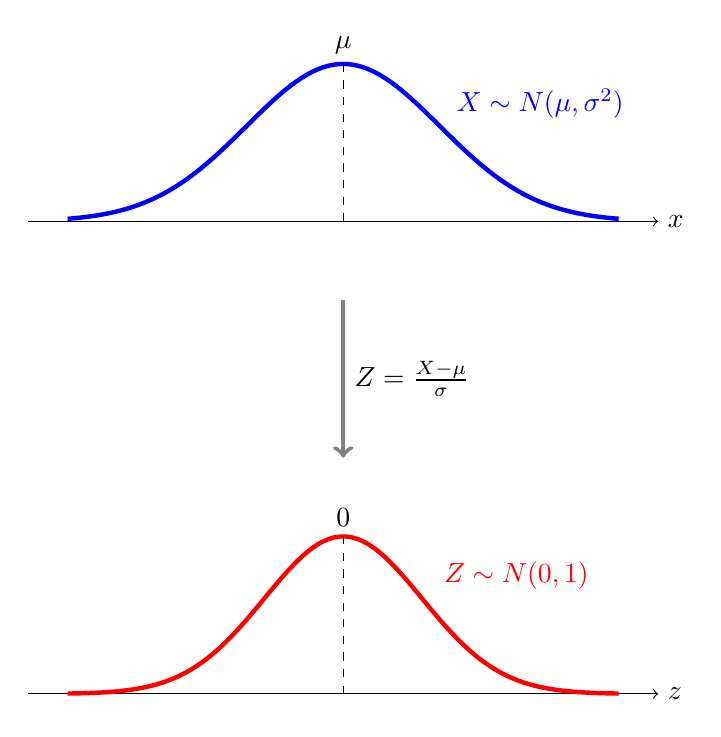
\begin{tikzpicture}
		% Top curve (X)
		\begin{scope}[shift={(0,6.0)}]
			\draw[->] (-4,0) -- (4,0) node[right] {$x$};
			\draw[blue, ultra thick] plot[domain=-3.5:3.5, samples=100] (\x, {2*exp(-\x*\x/3)});
			\draw[dashed] (0,0) -- (0,2) node[above] {$\mu$};
			\node[blue] at (2.5,1.5) {$X \sim N(\mu, \sigma^2)$};
		\end{scope}
		
		% Bottom curve (Z)
		\begin{scope}[shift={(0,0)}]
			\draw[->] (-4,0) -- (4,0) node[right] {$z$};
			\draw[red, ultra thick] plot[domain=-3.5:3.5, samples=100] (\x, {2*exp(-\x*\x/2)});
			\draw[dashed] (0,0) -- (0,2) node[above] {$0$};
			\node[red] at (2.2,1.5) {$Z \sim N(0, 1)$};
		\end{scope}
		
		% Transformation Arrow
		\draw[->, ultra thick, gray] (0, 5.0) -- (0, 3.0) node[midway, right, black] {$Z = \frac{X-\mu}{\sigma}$};
	\end{tikzpicture}
	\caption{Standardization of a Normal Distribution.}
\end{figure}

\newpage
\section{Normal Approximation of the Binomial Distribution}

Calculating binomial probabilities for large sample sizes ($n$) can be computationally exhausting. Fortunately, when certain conditions are met---specifically when $np > 5$ and $n(1-p) > 5$---the discrete Binomial Distribution $B(n, p)$ can be closely approximated by a Normal Distribution with $\mu = np$ and $\sigma^2 = np(1-p)$. \\

When performing this approximation, we must apply a ``continuity correction.'' Since we are using a continuous curve to model discrete steps, we adjust the boundaries by $0.5$. For example, to find the probability that $X$ is greater than 25 in a discrete sense, we calculate the area under the normal curve for $Y > 25.5$. This adjustment accounts for the fact that the discrete value ``25'' actually occupies the space from $24.5$ to $25.5$ in a continuous model.

\begin{figure}[H]
	\centering
	% TIKZ_PLACEHOLDER_5: A discrete binomial histogram overlaid with a smooth normal density curve, highlighting the 0.5 boundary shift.
	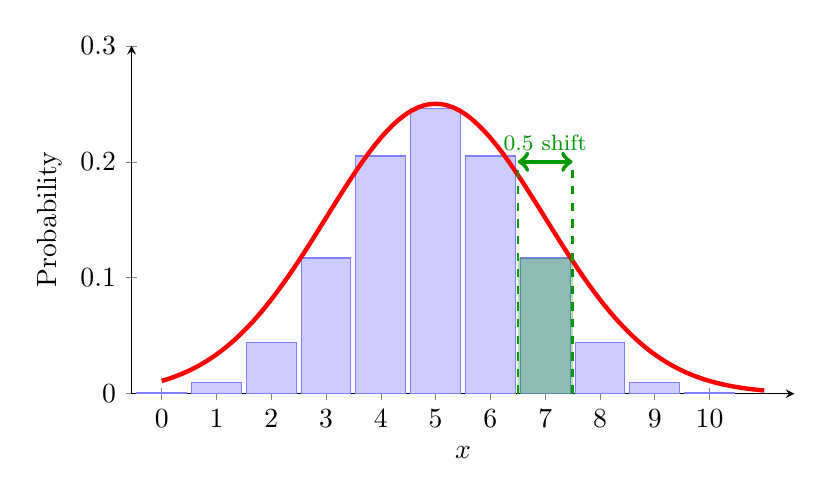
\begin{tikzpicture}
		\begin{axis}[
			ymin=0, ymax=0.3,
			xlabel=$x$,
			ylabel=Probability,
			height=6cm, width=10cm,
			xtick={0,1,2,3,4,5,6,7,8,9,10},
			domain=0:11,
			samples=12,
			axis lines=left,
			enlarge x limits=0.05
		]
			% Binomial-like bars
			\addplot[ybar, bar width=18pt, fill=blue!20, draw=blue!50] coordinates {
				(0,0.001) (1,0.010) (2,0.044) (3,0.117) (4,0.205) (5,0.246) (6,0.205) (7,0.117) (8,0.044) (9,0.010) (10,0.001)
			};
			
			% Normal curve overlay
			\addplot[red, ultra thick, samples=100, domain=0:11] {0.25*exp(-(x-5)^2/8)};
			
			% Continuity correction highlight at x=7
			\draw[<->, ultra thick, green!60!black] (axis cs:6.5, 0.2) -- (axis cs:7.5, 0.2) node[midway, above, font=\footnotesize] {0.5 shift};
			\draw[dashed, green!60!black, thick] (axis cs:6.5, 0) -- (axis cs:6.5, 0.2);
			\draw[dashed, green!60!black, thick] (axis cs:7.5, 0) -- (axis cs:7.5, 0.2);
			\fill[green!60!black, opacity=0.3] (axis cs:6.5,0) rectangle (axis cs:7.5,0.117);
		\end{axis}
	\end{tikzpicture}
	\caption{Fitting a normal curve to a binomial distribution.}
\end{figure}

\section{Combining Random Variables}

In many statistical applications, we need to consider the sum or difference of multiple random variables. If we have two independent variables $X$ and $Y$, the expected value of their sum or difference is simply the sum or difference of their individual expectations:
\begin{equation}
	E(aX \pm bY) = aE(X) \pm bE(Y)
\end{equation}

However, the rule for variance is different. Even when subtracting variables, the uncertainties (variances) always add, provided the variables are independent:
\begin{equation}
	Var(aX \pm bY) = a^2Var(X) + b^2Var(Y)
\end{equation}

If the original variables are normally distributed, their linear combination will also follow a normal distribution, allowing us to calculate probabilities for the combined outcome using the same Z-score techniques discussed earlier.

\begin{figure}[H]
	\centering
	% TIKZ_PLACEHOLDER_6: A diagram showing two separate normal curves X and Y combining into a new, wider normal curve T = X+Y.
	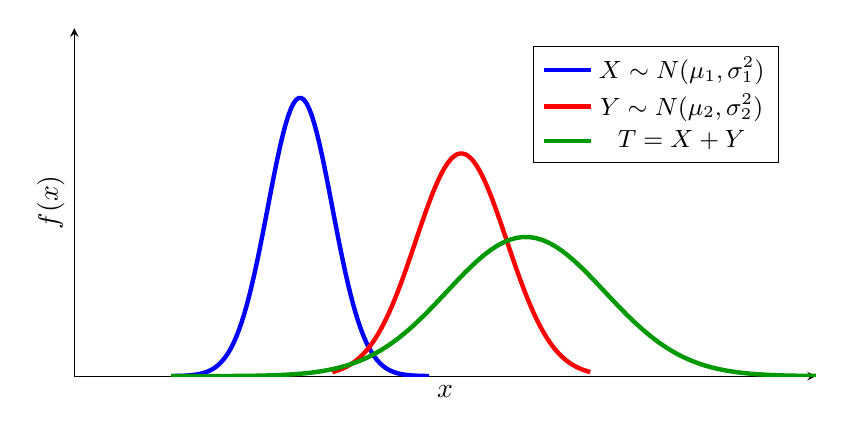
\begin{tikzpicture}
		\begin{axis}[
			axis lines = left,
			xlabel = $x$,
			ylabel = $f(x)$,
			ymin=0, ymax=0.5,
			xmin=-5, xmax=18,
			ticks=none,
			height=6cm, width=11cm,
			legend style={at={(0.95,0.95)}, anchor=north east, font=\small}
		]
			\addplot[ultra thick, blue, domain=-2:6, samples=100] {0.4*exp(-(x-2)^2/2)};
			\addlegendentry{$X \sim N(\mu_1, \sigma_1^2)$}
			
			\addplot[ultra thick, red, domain=3:11, samples=100] {0.32*exp(-(x-7)^2/4)};
			\addlegendentry{$Y \sim N(\mu_2, \sigma_2^2)$}
			
			\addplot[ultra thick, green!60!black, domain=-2:18, samples=100] {0.2*exp(-(x-9)^2/12)};
			\addlegendentry{$T = X+Y$}
		\end{axis}
	\end{tikzpicture}
	\caption{Sum of independent normal random variables.}
\end{figure}

\section{Statistical Studies and the Logic of Inference}

The ultimate goal of studying these distributions is to perform statistical inference---using data from a small sample to draw conclusions about a larger population. A population parameter (like the true mean $\mu$) is often unknown, so we calculate a sample statistic (like the sample mean $\bar{x}$) to estimate it. \\

The validity of these inferences depends heavily on the study design. In an \textbf{Observational Study}, researchers simply observe and measure participants without intervention. While these studies are excellent for establishing \textbf{correlation} (showing that two variables move together), they cannot establish \textbf{causation} due to the potential influence of ``lurking variables.'' To establish a cause-and-effect relationship, a \textbf{Randomized Controlled Experiment} is required, where participants are randomly assigned to a treatment or control group to isolate the effect of the variable being studied.

\begin{figure}[H]
	\centering
	% TIKZ_PLACEHOLDER_7: A flowchart branching from 'Study Designs' into 'Descriptive/Survey' (No comparison) and 'Analytic' (Comparison), then splitting 'Analytic' into 'Observational' and 'Experimental'.
	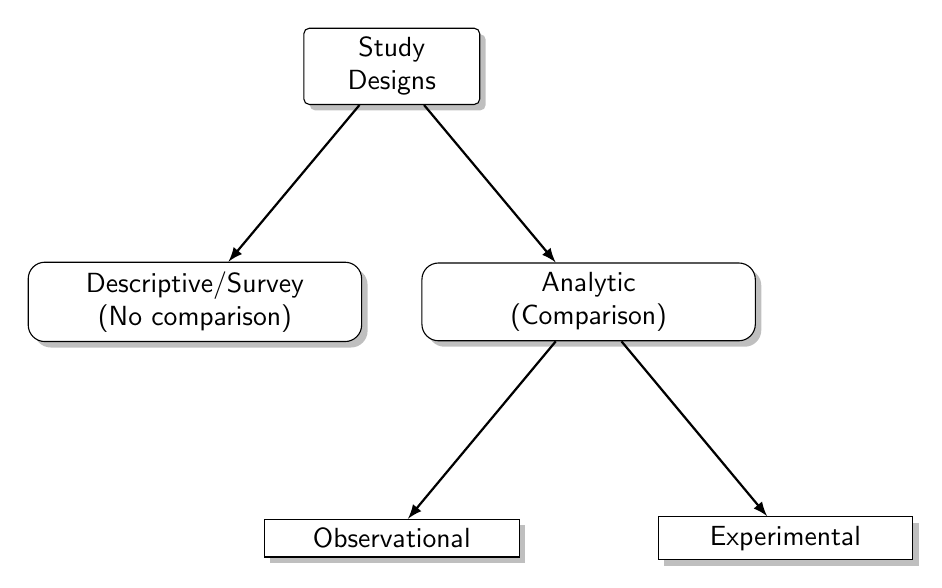
\begin{tikzpicture}[
		edge from parent/.style={draw, thick, -latex},
		level distance=2.5cm,
		sibling distance=5cm,
		growth parent anchor=south
	]
		\usetikzlibrary{shadows}
		\node[root] {Study Designs}
			child {node[level-2] {Descriptive/Survey\\(No comparison)}}
			child {node[level-2] {Analytic\\(Comparison)}
				child {node[level-3] {Observational}
					edge from parent [sibling distance=3cm]
				}
				child {node[level-3] {Experimental}
					edge from parent [sibling distance=3cm]
				}
			};
	\end{tikzpicture}
	\caption{Categorization of statistical studies.}
\end{figure}

\end{document}
